\chapter{BMA Posterior Distributions}\label{appendix1}
\fixchapterheading

\vspace{0.8cm}

An alternative method for graphically representing model specification uncertainty and coefficient magnitude uncertainty is the plotting of the posterior distributions for the coefficients.  In Table 5.2, the posterior probability that the variable belongs to the best model and the expected value of the coefficient were given numerically for each variable.  The plot in Figure 5.2 gave expression to the posterior probabilities associated with each variable by showing the frequency with which the variables appear in the best models.  While Figure 5.2 produces only a graphical representation of the posterior probabilities that variables are members of the best model, the posterior probability distributions for the coefficients in Figures A.1 and A.2 simultaneously express the posterior probabilities that the variables belong to the best model and the expected values of the coefficients.

A posterior coefficient distribution is produced for each of the 37 variables and the intercept term in Figures A.1 and A.2.  Each distribution is centered over the expected value of coefficient and is scaled so that its maximum height is equal to the probability that the variable is a member of the best model.   A spike is centered at zero in each distribution and its height expresses the probability that the variable is not a member of the best model.  The sum of the maximum height of the distribution and the height of the spike is one.  Together, Figures A.1 and A.2 provide a complete graphical representation of the posterior probability, expected value, and standard deviation columns in Table 5.2 for all of the variables.


\begin{figure}[t]
\begin{center}
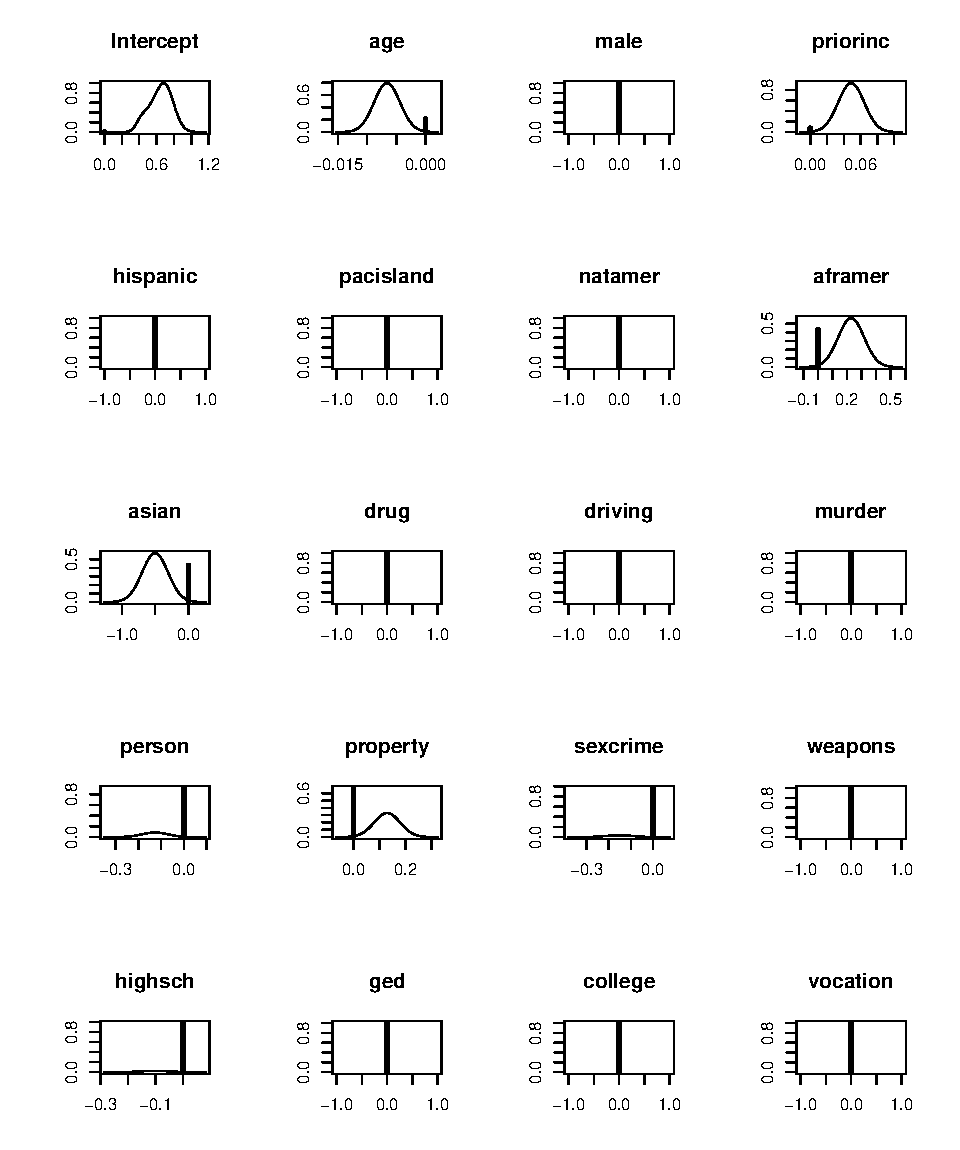
\includegraphics[height=20cm,width=14.5cm]{graphapp031.eps}
\caption{Posterior Distributions for the Intercept and Variables 1-19}
\end{center}
\end{figure}

\begin{figure}[t]
\begin{center}
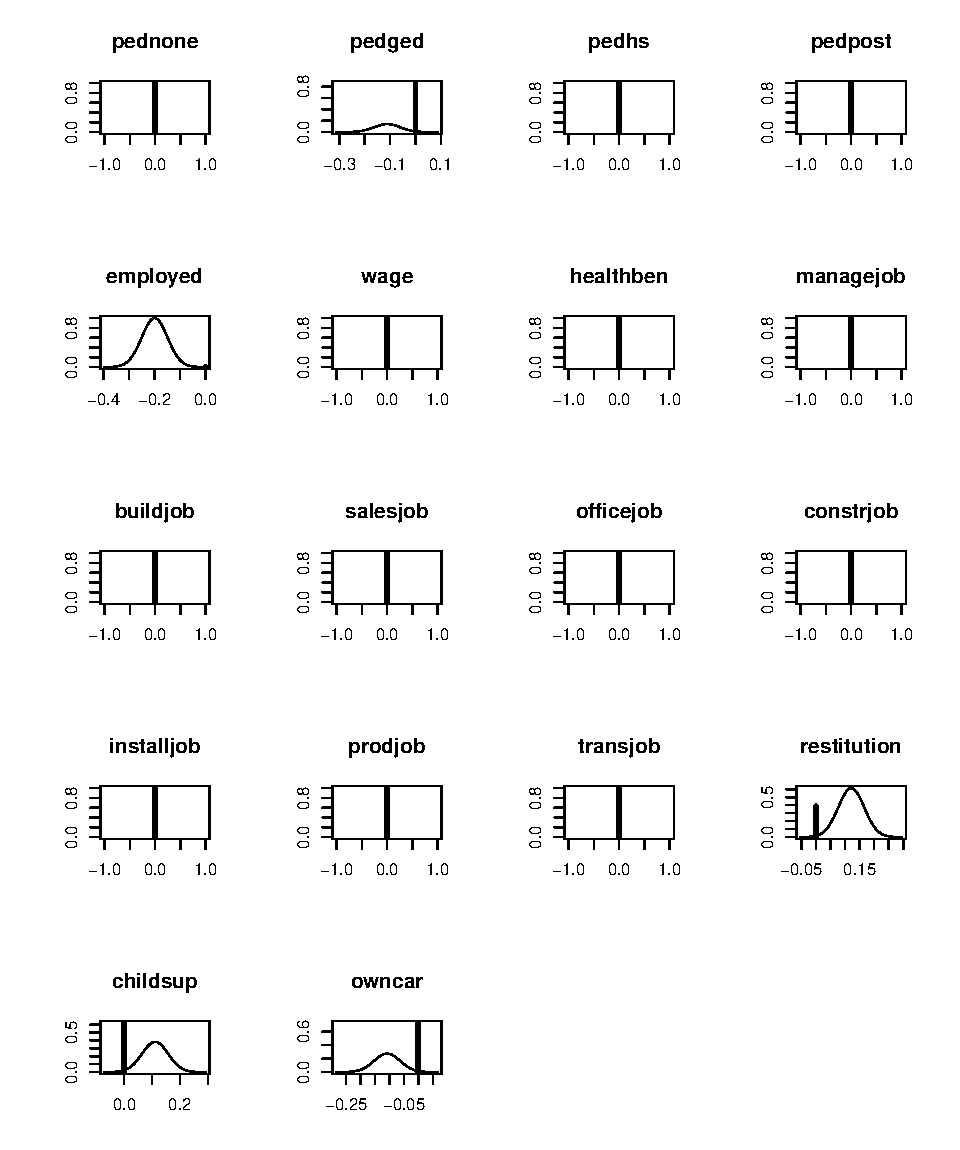
\includegraphics[height=20cm,width=14.5cm]{graphapp032.eps}
\caption{Posterior Distributions for Variables 20-37}
\end{center}
\end{figure}



%\begin{figure}[t]
%\begin{center}
%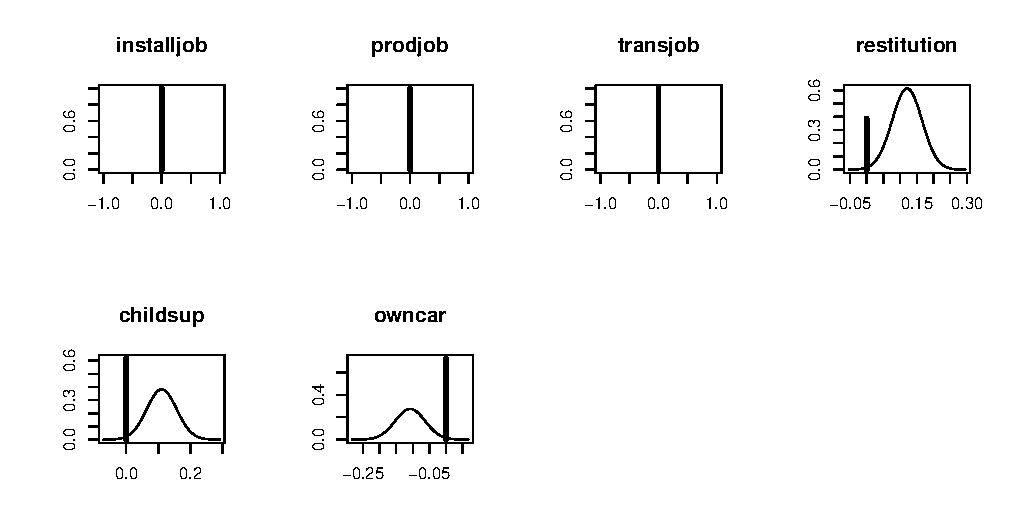
\includegraphics[clip=true,viewport=0mm 0mm 168mm 180mm, scale=0.85]{graphapp013.eps}
%\caption{Posterior Distributions for Variable 32-37}
%\end{center}
%\end{figure}
